Es gibt eine Reihe von Definitionen für den Begriff Automatisierung. Aus dem Gabler Wirtschaftslexikon und dem Duden gehen hervor, dass es sich dabei um die Idee handelt, Maschinen einzusetzen, die bestimmte Tätigkeiten übernehmen, welche sonst durch Menschen ausgeführt würden\footnote{\cite{Dudenredaktion.2023}} \footnote{\cite{.2019}}.

Abzugrenzen ist dieser Begriff von einen reinen technologischen Unterstützung, bei der menschliche Tätigkeiten lediglich unterstützt, jedoch nicht vollständig übernommen werden. Beispielsweise handelt es sich bei Sturzerkennungssystemen, die in der Altenpflege eingesetzt werden, um Stürze zu erkennen und bei Bedarf Pflegepersonal oder Angehörige zu informieren, nicht um Automatisierung, sondern lediglich um eine technologische Unterstützung\footnote{Vgl. \cite{Ganyo.2011}, S. 1354 f.}.

% auch das ADAC grenzt Fahrerassistenz und Automatisierung auf ähnliche Weise ab

In den vergangenen Jahren sind einige Technologien zur Automatisierung aufgekommen, die die Arbeitswelt stark beeinflussen. Dazu gehören beispielsweise Roboter, die bestimmte Fertigungsprozesse vollständig übernehmen oder KI Systeme, die in Bewerbungsprozessen Entscheidungen über die Auswahl von Bewerbern treffen.\footnote{Vgl. \cite{DagnyDukach.2022}}.

% Industrieroboter bereits seit Jahrzehnten

Die Motivation hinter Automatisierung liegt meistens darin, die Kosten für die Durchführung der automatisierten Tätigkeiten zu senken. Das geht häufig mit einem Wandel, häufig auch mit einem Verlust von Arbeitsplätzen einher. Durch Automatisierung können auch neue Arbeitsplätze entstehen. Je nach Branche reicht dies häufig jedoch nicht aus, um den Verlust auszugleichen. Außerdem sind die neu entstehenden Berufe oftmals mit erhöhten Qualifikationisanforderungen verbunden\footnote{\cite{DagnyDukach.2022}} \footnote{\cite{Dengler.2019}}. Daher führen Entwicklungen dieser Art bei vielen Menschen zu zunehmender Besorgnis um die Qualität und die Existenz ihrer Arbeitsplätze\footnote{Vgl. \cite{AaronSmith.2017}}. 

Verschiedene Berufe lassen sich unterschiedlich gut automatisieren. Das IAB hat für verschiedene Berufssegmente Substituierungspotenziale berechnet, die den Anteil der darin ausgeübten Tätigkeiten beschreiben, die automatisiert werden können. Bei Fertigungsberufen ist dieser Anteil mit 83\% in 2016 besonders groß. Soziale und kulturelle Diensleistungsberufe haben mit 13\% ein sehr niedriges Substituierbarkeitspotenzial. Ein mittleres Substituierbarkeitspotenzial von 40\% weisen Lebensmittel- und Gastgewerbeberufe auf\footnote{\cite{Dengler.2019}, S. 10}. Es ist wichtig zu beachten, dass die in dieser Grafik dargestellten Daten zuletzt im Jahr 2019 aktualisiert wurden und sich seitdem insbesondere im Bereich der KI bedeutende Entwicklungen ereignet haben.

\begin{figure}[]
  \centering
  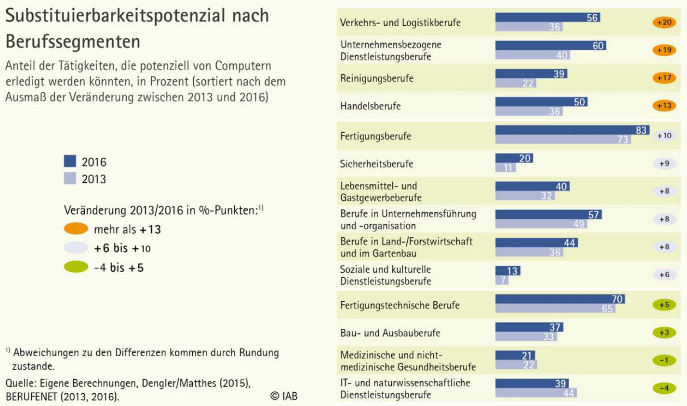
\includegraphics[width=0.95\textwidth]{Bilder/iab-substituierbarkeitspotenzial.png}
  \caption{Substituierbarkeitspotenzial nach Berufssegmenten (Dengler, 2019, S. 10)}
  \label{fig:bildlabel}
\end{figure}

\newpage

Die Folgen der Automatisierung in den jeweiligen Berufssegmenten unterscheiden sich und es liegt nahe, dass beim ethischen Umgang mit Automatisierung auf verschiedene Dinge geachtet werden muss.
